\documentclass[titlepage]{article}

\usepackage[letterpaper,margin=1in,footskip=0.25in]{geometry}
\usepackage{fancyhdr}
\usepackage{amsmath}
\usepackage{mathtools}
\usepackage{tikz}
\usepackage{subcaption}
\usepackage{float}
\usepackage{csquotes}
\usepackage[hidelinks]{hyperref}
\usepackage{scrextend}

\colorlet{grx}{green!50!black}
\colorlet{blx}{blue!80!green!70}

\MakeOuterQuote{"}

\deffootnotemark{\textsuperscript{[\thefootnotemark]}}
\deffootnote{2em}{1.6em}{\textsuperscript{\thefootnotemark}}

\pagestyle{fancy}
\fancyhf{}
\rfoot{Labalme \thepage}
\renewcommand{\headrulewidth}{0pt}

\begin{document}




\noindent Steven Labalme\\
\noindent Mr. Bilak\\
\noindent AP Physics C: Electricity and Magnetism, 6\\
\noindent 19 March 2020\\
\begin{center}
    \section*{An Analysis of the Electric Potential of Two Point Charges}
\end{center}

\begin{figure}[h!]
    \centering
    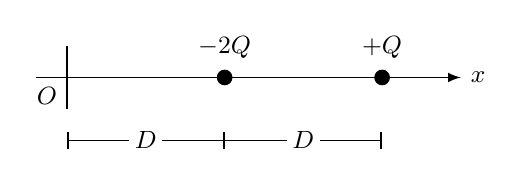
\begin{tikzpicture}[
        scale=2,
        charge/.style={circle,fill,inner sep=2pt,label={above:\small$#1$}},
        every path/.append style={semithick}
    ]
        \draw [-latex] (-0.2,0) -- (2.5,0) node[right]{\small$x$};
        \draw (0,-0.2) -- node[below left]{\small$O$} (0,0.2);

        \node [charge=+Q]  at (2,0) {};
        \node [charge=-2Q] at (1,0) {};

        \draw [|-|] (0,-0.4) -- node[fill=white,inner sep=2pt]{\small$D$} (1,-0.4);
        \draw [-|]  (1,-0.4) -- node[fill=white,inner sep=2pt]{\small$D$} (2,-0.4);
    \end{tikzpicture}
    \caption{Two point charges along the $x$ axis.}
    \label{fig:2charges}
\end{figure}

\subsection*{Motivation and Goal}
Generalize Question 49 of Section I of the 1993 AP Physics C: Electricity and Magnetism examination to the following: given Figure \ref{fig:2charges}, find the distance from the origin $O$ to all points along the $x$-axis where the net electric potential is equal to zero.\par
There is a conventional way to solve this type of problem that unfortunately lacks much of a connection to conceptual physics. This method will be explored first, along with its shortcomings. To correct its mistakes, a second method will be proposed, applying a mathematical model that captures the underlying physics with greater clarity. Two methods of solving this second model will be explored --- a simple but redundant method, and a more elegant algorithm.\par
Lastly, a surprising connection between the first and the second method will be explored.


\subsection*{The Conventional Method}
The electric potential, or voltage $V$, given as a function of the linear distance $r$ from a point charge of magnitude $q$ and fundamental constants is given by the following.
\begin{equation*}
    V=\frac{kq}{r}
\end{equation*}
Thus, the voltage along the $x$-axis caused solely by the point charge of magnitude $+Q$ a distance $r$ from said charge is $$V=\frac{kQ}{r}$$Likewise, the voltage along the $x$-axis caused solely by the point charge of magnitude $-2Q$ a distance $r'$ from said charge is $$V'=\frac{k(-2Q)}{r'}=\frac{-2kQ}{r'}$$As is implied by the notation\footnote{This is very important to recognize.}, $r\neq r'$. Indeed, the two voltage functions operate on \emph{distinct} coordinate systems; because $r$ and $r'$ are distances \emph{relative} to their respective point charges, \emph{they have no bearing on each other}.\par
Of course, in order to solve the problem, $r$ and $r'$ must be related to each other. Furthermore, they must be related to the absolute coordinate system determined by the set placement of the origin. Therefore, it is necessary to find $r$ and $r'$ as a function of a distance $x$ from the origin along the $x$-axis. Consider Figure \ref{fig:rAndrPrime} to help visualize this goal.

\begin{figure}[h!]
    \centering
    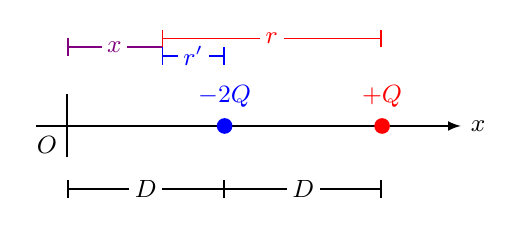
\begin{tikzpicture}[
        scale=2,
        colorcharge/.style 2 args={circle,fill,#2,inner sep=2pt,label={above:\small${\color{#2}#1}$}},
        every path/.append style={semithick}
    ]
        \draw [-latex] (-0.2,0) -- (2.5,0) node[right]{\small$x$};
        \draw (0,-0.2) -- node[below left]{\small$O$} (0,0.2);

        \draw [|-|] (0,-0.4) -- node[fill=white,inner sep=2pt]{\small$D$} (1,-0.4);
        \draw [-|]  (1,-0.4) -- node[fill=white,inner sep=2pt]{\small$D$} (2,-0.4);

        \node [colorcharge={+Q}{red}]   at (2,0) {};
        \node [colorcharge={-2Q}{blue}] at (1,0) {};

        \draw [red!50!blue,|-] (0,0.5)   -- node[fill=white,inner sep=2pt]{\small$x$}  (0.6,0.5);
        \draw [red,|-|]        (0.6,0.555) -- node[fill=white,inner sep=2pt]{\small$r$}  (2,0.555);
        \draw [blue,|-|]       (0.6,0.445) -- node[fill=white,inner sep=2pt]{\small$r'$} (1,0.445);
    \end{tikzpicture}
    \caption{Relating $r$ and $r'$ to $O$.}
    \label{fig:rAndrPrime}
\end{figure}

From Figure \ref{fig:rAndrPrime}, the following two relationships are immediately evident.
\begin{align*}
    x+r &= 2D\\
    x+r' &= D
\end{align*}
From the above two equations, solve for $r$ and $r'$, respectively, and substitute into the above equations for $V$ and $V'$.
\begin{align*}
    r &= 2D-x\\
    r' &= D-x
\end{align*}
\begin{align}
    V &= \frac{kQ}{2D-x}\label{eqn:Vinitial}\\
    V' &= \frac{-2kQ}{D-x}\label{eqn:VprimeInitial}
\end{align}

Although it may not seem like it, Equations \ref{eqn:Vinitial} and \ref{eqn:VprimeInitial} constitute a substantial advance toward solving the problem. Indeed, they relate all of the information given in the question ($D$, $+Q$, $-2Q$, and, albeit indirectly, the position of the origin) with the sought-after value ($x$). All that's left to recognize is the condition(s) that $V$ and $V'$ must satisfy and to solve for $x$. Unfortunately, this is where this method diverges from conceptually justifiable mathematical manipulations.\par
From the question, it appears that $V$ and $V'$ must satisfy $$\sum V=V+V'=0$$ However, $$V-V'=0$$ oddly gives another valid solution. Substituting and solving gives the following two values for $x$ and solutions to the problem.
\begin{align*}
    V+V' &= 0&
        V-V' &= 0\\
    \frac{kQ}{2D-x}+\frac{-2kQ}{D-x} &= 0&
        \frac{kQ}{2D-x}-\frac{-2kQ}{D-x} &= 0\\
    \frac{kQ}{2D-x} &= \frac{2kQ}{D-x}&
        \frac{kQ}{2D-x} &= \frac{-2kQ}{D-x}\\
    \frac{1}{2D-x} &= \frac{2}{D-x}&
        \frac{1}{2D-x} &= \frac{-2}{D-x}\\
    (1)(D-x) &= (2)(2D-x)&
        (1)(D-x) &= (-2)(2D-x)\\
    D-x &= 4D-2x&
        D-x &= -4D+2x\\
    \Aboxed{x &= 3D}&
        5D &= 3x\\
    &&
        \Aboxed{x &= \frac{5}{3}D}
\end{align*}

\begin{figure}[H]
    \centering
    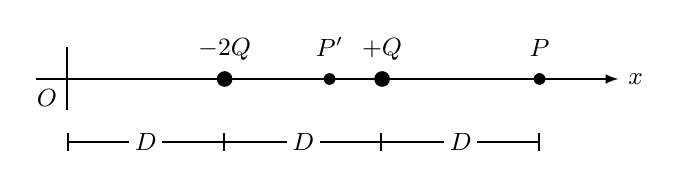
\begin{tikzpicture}[
        scale=2,
        charge/.style={circle,fill,inner sep=2pt,label={above:\small$#1$}},
        point/.style={circle,fill,inner sep=1.5pt,label={[yshift=2pt]above:\small$#1$}},
        every path/.append style={semithick}
    ]
        \draw [-latex] (-0.2,0) -- (3.5,0) node[right]{\small$x$};
        \draw (0,-0.2) -- node[below left]{\small$O$} (0,0.2);

        \node [charge=+Q]  at (2,0) {};
        \node [charge=-2Q] at (1,0) {};
        \node [point=P] at (3,0) {};
        \node [point=P'] at ({5/3},0) {};

        \draw [|-|] (0,-0.4) -- node[fill=white,inner sep=2pt]{\small$D$} (1,-0.4);
        \draw [-|]  (1,-0.4) -- node[fill=white,inner sep=2pt]{\small$D$} (2,-0.4);
        \draw [-|]  (2,-0.4) -- node[fill=white,inner sep=2pt]{\small$D$} (3,-0.4);
    \end{tikzpicture}
    \caption{The solutions to the problem.}
    \label{fig:2points}
\end{figure}

Graphically, these points would fall along the $x$-axis at the points $P$ and $P'$, as shown in Figure \ref{fig:2points}. Considering Figure \ref{fig:2points} may well convince the reader that the above solutions (and only the above solutions) are valid, even if doubt about the mechanics of this conventional method persists.

\subsubsection*{Shortcomings}
The major issue with the conventional method was already referenced: The seemingly inexplicable fact that $V-V'=0$ gives a valid solution. However, there is another problem, which partially explains the previous issue: Distance from a point charge is always a positive number, yet $2D-x$ and $D-x$, which the conventional method sets \emph{equal} to $r$ and $r'$, respectively, return negative outputs for many values of $x$.\par
This second problem is clarified when $V$ and $V'$ are considered graphically (see Figure \ref{fig:VVprimeGraph}).

\begin{figure}[h!]
    \centering
    \begin{subfigure}[b]{0.45\linewidth}
        \centering
        \begin{tikzpicture}[
            yscale=0.2
        ]
            \draw [-latex,semithick] (-1.5,0) -- (4.5,0) node[right]{\small$x$};
            \draw [-latex,semithick] (0,-20) -- (0,20) node[above]{\small$V$};

            \draw [dashed] (2,-20) -- (2,20);

            \foreach \x in {-1,1,2,3,4} {
                \draw (\x,-0.5) node[below,fill=white]{\footnotesize$\x D$} -- (\x,0.5);
            }

            \clip (-1.5,-20) rectangle (4.5,20);
            \draw [orange,thick,domain=-1.5:1.96,samples=500,smooth] plot ({\x},{1/(2-\x)});
            \draw [orange,thick,domain=2.04:4.5,samples=500,smooth] plot ({\x},{1/(2-\x)});
        \end{tikzpicture}
        \caption{$V$}
        \label{fig:VVprimeGrapha}
    \end{subfigure}
    \begin{subfigure}[b]{0.45\linewidth}
        \centering
        \begin{tikzpicture}[
            yscale=0.2
        ]
            \draw [-latex,semithick] (-1.5,0) -- (4.5,0) node[right]{\small$x$};
            \draw [-latex,semithick] (0,-20) -- (0,20) node[above]{\small$V'$};

            \draw [dashed] (1,-20) -- (1,20);

            \foreach \x in {-1,1,2,3,4} {
                \draw (\x,-0.5) node[below,fill=white]{\footnotesize$\x D$} -- (\x,0.5);
            }

            \clip (-1.5,-20) rectangle (4.5,20);
            \draw [grx,thick,domain=-1.5:0.92,samples=500,smooth] plot ({\x},{-2/(1-\x)});
            \draw [grx,thick,domain=1.08:4.5,samples=500,smooth] plot ({\x},{-2/(1-\x)});
        \end{tikzpicture}
        \caption{$V'$}
        \label{fig:VVprimeGraphb}
    \end{subfigure}
    \caption{Graphs of $V$ and $V'$.}
    \label{fig:VVprimeGraph}
\end{figure}

In Figure \ref{fig:VVprimeGrapha}, the voltage should converge on $+\infty$ from both sides of the asymptote due to the positive nature of the charge, $+Q$. Similarly, in Figure \ref{fig:VVprimeGraphb}, the voltage should converge on $-\infty$ from both sides of the asymptote due to the negative nature of the charge, $-2Q$.\par
It is precisely this problem that necessitates the use of both $V+V'=0$ and $V-V'=0$ (see Figure \ref{fig:connectingGrapha} for their graphs). Essentially, considering both $V+V'$ and $V-V'$ works around the sign issues present in Figure \ref{fig:VVprimeGraph}, allowing both solutions to be obtained.


\subsection*{Developing a New Method}
Since the only issue with $r=2D-x$ and $r'=D-x$ is that the quantities are occasionally negative, take the absolute value of both quantities. This will yield the following new equations for $V$ and $V'$.
\begin{align}
    V &= \frac{kQ}{|2D-x|}\label{eqn:Vnew}\\
    V' &= \frac{-2kQ}{|D-x|}\label{eqn:VprimeNew}
\end{align}
This change has already solved both of the previously referenced problems. Now, when the net electric potential $\sum V = V+V'$ is graphed, the resultant function has two $x$-intercepts in the appropriate places (see Figure \ref{fig:absGraph}). It also accurately captures the full picture of the "absolute" voltage along the $x$-axis.

\begin{figure}[h!]
    \centering
    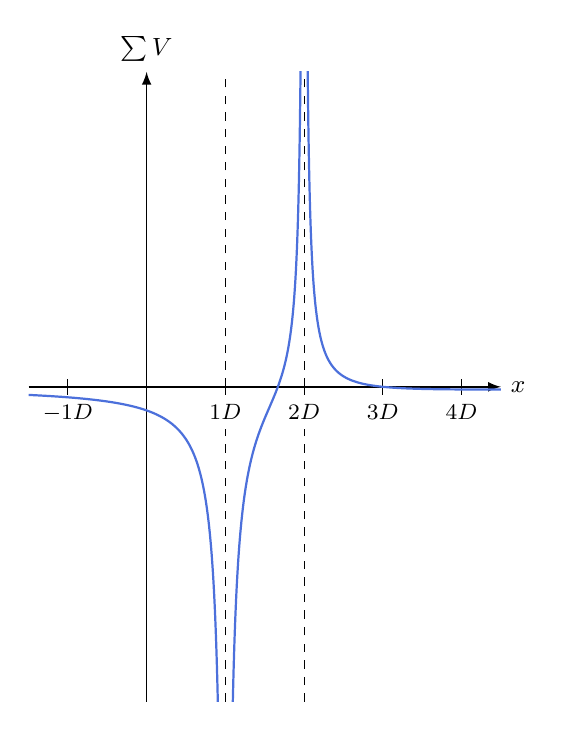
\begin{tikzpicture}[
        yscale=0.2
    ]
        \draw [-latex,semithick] (-1.5,0) -- (4.5,0) node[right]{\small$x$};
        \draw [-latex,semithick] (0,-20) -- (0,20) node[above]{\small$\sum V$};

        \draw [dashed] (1,-20) -- (1,20);
        \draw [dashed] (2,-20) -- (2,20);

        \foreach \x in {-1,1,2,3,4} {
            \draw (\x,-0.5) node[below,fill=white]{\footnotesize$\x D$} -- (\x,0.5);
        }

        \clip (-1.5,-20) rectangle (4.5,20);
        \draw [blx,thick,domain=-1.5:0.92,samples=500,smooth] plot ({\x},{1/(2-\x)-2/(1-\x)});
        \draw [blx,thick,domain=1.08:1.96,samples=500,smooth] plot ({\x},{1/(2-\x)+2/(1-\x)});
        \draw [blx,thick,domain=2.04:4.5,samples=500,smooth] plot ({\x},{2/(1-\x)-1/(2-\x)});
    \end{tikzpicture}
    \caption{A graph of the correct $\sum V$.}
    \label{fig:absGraph}
\end{figure}

Thus, all that remains is to algebraically solve $\sum V = 0$. This paper will explore, and contrast, two ways to do so.

\subsubsection*{Expanding the Absolute Value Expressions}
Begin with the following statement, which both Figure \ref{fig:absGraph} and the evaluation of the conventional method demonstrate can be solved for two distinct values of $x$.
\begin{equation*}
    \frac{kQ}{|2D-x|}+\frac{-2kQ}{|D-x|}=0
\end{equation*}
Simplify to remove extraneous terms and eliminate the fractions.
\begin{align*}
    \frac{kQ}{|2D-x|} &= \frac{2kQ}{|D-x|}\\
    |D-x| &= 2|2D-x|\stepcounter{equation}\tag{\theequation}\label{eqn:abs}
\end{align*}
To evaluate $|f|$, where $f$ is some function, write two new equations. One of these new equations will have $f$ substituted for $|f|$, and the other will have $-f$ substituted for $|f|$. Thus, since each absolute value splits an equation into two, and there are two absolute value expressions present in Equation \ref{eqn:abs}, it will split into four parts. Each of these four parts can, in turn, be solved for a value of $x$. Note that since only two distinct answers are to be expected from the four equations, there will be some redundancy involved in these calculations.\par
The division of Equation \ref{eqn:abs} is visually captured in Figure \ref{fig:tree}\footnote{Note that switching the order of a difference of two terms is another way of multiplying it by $-1$.}.

\begin{figure}[h!]
    \centering
    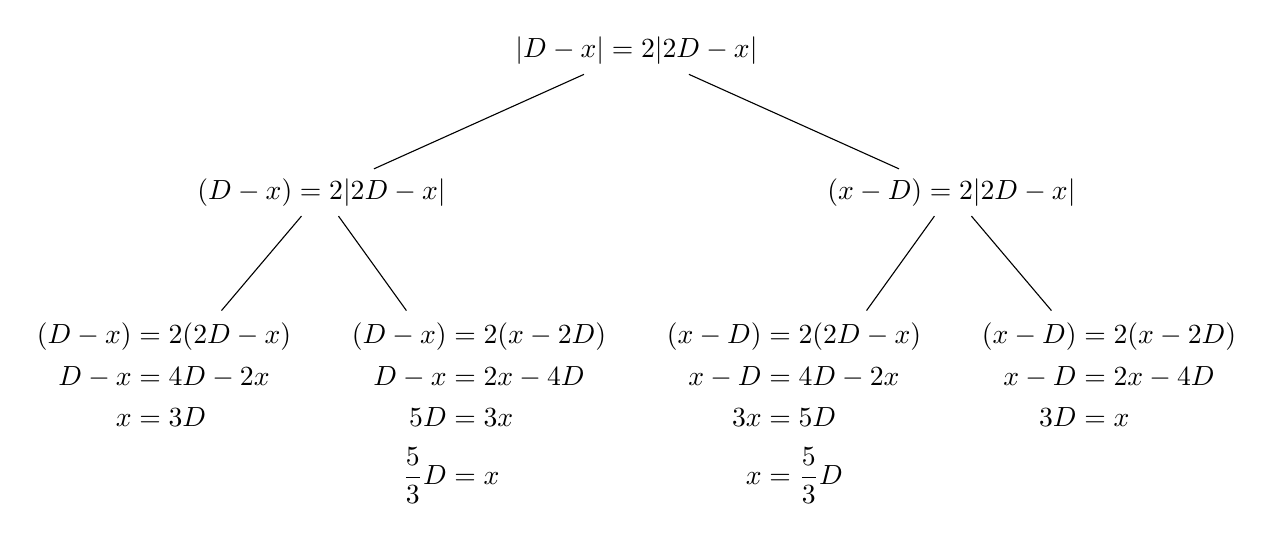
\begin{tikzpicture}[
        level/.style={sibling distance=8cm/#1},
        every node/.style={anchor=north}
    ]
        \node {$|D-x|=2|2D-x|$}
            child {node {$(D-x)=2|2D-x|$}
                child {node {$
                    \begin{aligned}
                        (D-x) &= 2(2D-x)\\
                        D-x &= 4D-2x\\
                        x &= 3D
                    \end{aligned}
                $}}
                child {node {$
                    \begin{aligned}
                        (D-x) &= 2(x-2D)\\
                        D-x &= 2x-4D\\
                        5D &= 3x\\
                        \frac{5}{3}D &= x
                    \end{aligned}
                $}}
            }
            child {node {$(x-D)=2|2D-x|$}
                child {node {$
                    \begin{aligned}
                        (x-D) &= 2(2D-x)\\
                        x-D &= 4D-2x\\
                        3x &= 5D\\
                        x &= \frac{5}{3}D
                    \end{aligned}
                $}}
                child {node {$
                    \begin{aligned}
                        (x-D) &= 2(x-2D)\\
                        x-D &= 2x-4D\\
                        3D &= x
                    \end{aligned}
                $}}
            }
        ;
    \end{tikzpicture}
    \caption{Splitting the absolute value expressions.}
    \label{fig:tree}
\end{figure}

As expected, each solution appears twice in Figure \ref{fig:tree}. Although it may not be immediately obvious, the connection between like solutions is that the starting points in the bottom row are the same equation, but with both sides multiplied by $-1$ (which, of course, does conserve equality). For example, $-(D-x)=-2(x-2D)$ is the same as $(x-D)=2(2D-x)$.\par
To eliminate the repetition in other problems of this type, any pair of distinct pathways could be eliminated. However, this is a rather unscientific process, so it is probably better to deal with the extra work.

\subsubsection*{Factoring a Binomial}
Although the above method of evaluating $\sum V = 0$ is certainly better than the conventional method, it is still imperfect due to the unnecessary calculations. To tidy up the algorithm for evaluating Equation \ref{eqn:abs}\footnote{Start here instead of at the beginning of the previous section because it is with the absolute values in Equation \ref{eqn:abs} that the problems emerge.}, make an assumption: Where there are two solutions, there is a binomial.\par
Consider how to find such a binomial. For starters, realize that it is necessary to ensure that $D-x$ and $2D-x$ always return positive values. However, they need not return their magnitude, exactly, per se. Therefore, let's consider other methods of ensuring positive values for $D-x$ and $2D-x$. One such way is to square them. Therefore, try squaring both sides of Equation \ref{eqn:abs}, yielding the following\footnote{The absolute values have been removed because they are unnecessary, given the squaring.}.
\begin{equation*}
    (D-x)^2=4(2D-x)^2
\end{equation*}
The above equation is exactly what is desired, although it may not look it. When expanded, the reader should be able to tell that a binomial in $x$ will result. This binomial can be factored to find the solutions, as follows.
\begin{align*}
    D^2-2Dx+x^2 &= 4(4D^2-4Dx+x^2)\\
    x^2-2Dx+D^2 &= 4x^2-16Dx+16D^2\\
    0 &= 3x^2-14Dx+15D^2\stepcounter{equation}\tag{\theequation}\label{eqn:binomial}\\
    0 &= (3x-5D)(x-3D)\stepcounter{equation}\tag{\theequation}\label{eqn:factors}
\end{align*}
The transition from Equation \ref{eqn:binomial} to \ref{eqn:factors} may not be immediately obvious to everyone. Remember, though: If in doubt, one can always resort to the quadratic formula.\par
As was expected, squaring both sides of Equation \ref{eqn:abs} yielded a binomial that could be factored. By the zero-product property, all that remains to solve for $x$ is to set both of the factors in the last step of the above series of equations equal to zero and solve, as follows.
\begin{align*}
    3x-5D &= 0&
        x-3D &= 0\\
    3x &= 5D&
        \Aboxed{x &= 3D}\\
    \Aboxed{x &= \frac{5}{3}D}
\end{align*}

\subsubsection*{Reflections on the New Method}
Because all steps can be justified using an accurate mathematical model, this new method is superior to the conventional method. To begin, the new method accurately captures voltage along the $x$-axis through the use of absolute value expressions (Equations \ref{eqn:Vnew} and \ref{eqn:VprimeNew}). The perks of only using one model as opposed to two are captured by Figure \ref{fig:absGraph}, which contains both $x$-intercepts and realistically models the voltage's positive and negative spikes. In addition to the improved conceptual model, arriving at Equation \ref{eqn:abs} is simple, and directly expanding its absolute value expressions provides a series of easy-to-solve, linear equations, displayed in Figure \ref{fig:tree}. Lastly, a more rigorous, systematic method of solving Equation \ref{eqn:abs} exists in factoring a binomial.\par
As a parting comment, relating this problem to a binomial means that the very well understood properties of polynomials can be applied to this problem, possibly generating mathematical predictions concerning the nature of the voltage of point particles.


\subsection*{Connecting the Conventional and the New Methods}
The conventional method provides two equations (Equations \ref{eqn:Vinitial} and \ref{eqn:VprimeInitial}), each of which has one zero, or $x$-intercept. Considering $V$ and $V'$ as defined by these equations, $V+V'$ and $V-V'$ can be graphically represented by the orange and green curves, respectively, in Figure \ref{fig:connectingGrapha}.

\begin{figure}[h!]
    \centering
    \begin{subfigure}[b]{0.45\linewidth}
        \centering
        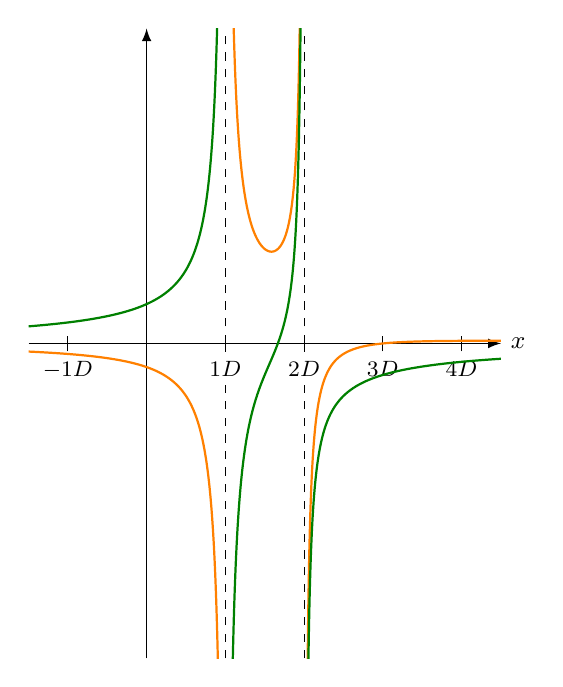
\begin{tikzpicture}[
            yscale=0.2
        ]
            \draw [-latex,semithick] (-1.5,0) -- (4.5,0) node[right]{\small$x$};
            \draw [-latex,semithick] (0,-20) -- (0,20);
    
            \draw [dashed] (1,-20) -- (1,20);
            \draw [dashed] (2,-20) -- (2,20);
    
            \foreach \x in {-1,1,2,3,4} {
                \draw (\x,-0.5) node[below,fill=white]{\footnotesize$\x D$} -- (\x,0.5);
            }
    
            \clip (-1.5,-20) rectangle (4.5,20);
            \draw [orange,thick,domain=-1.5:0.92,samples=500,smooth] plot ({\x},{1/(2-\x)-2/(1-\x)});
            \draw [orange,thick,domain=1.08:1.96,samples=500,smooth] plot ({\x},{1/(2-\x)-2/(1-\x)});
            \draw [orange,thick,domain=2.04:4.5,samples=500,smooth] plot ({\x},{1/(2-\x)-2/(1-\x)});
            \draw [grx,thick,domain=-1.5:0.92,samples=500,smooth] plot ({\x},{1/(2-\x)+2/(1-\x)});
            \draw [grx,thick,domain=1.08:1.96,samples=500,smooth] plot ({\x},{1/(2-\x)+2/(1-\x)});
            \draw [grx,thick,domain=2.04:4.5,samples=500,smooth] plot ({\x},{1/(2-\x)+2/(1-\x)});
        \end{tikzpicture}
        \caption{$V+V'$ in orange and $V-V'$ in green.}
        \label{fig:connectingGrapha}
    \end{subfigure}
    \begin{subfigure}[b]{0.45\linewidth}
        \centering
        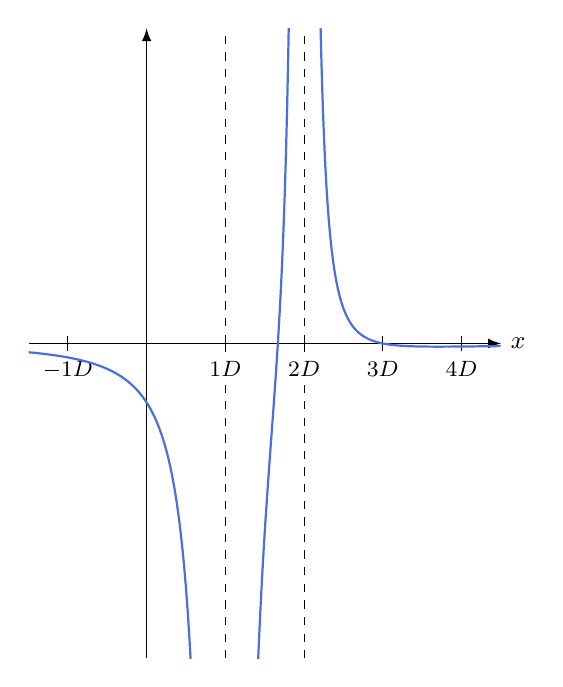
\begin{tikzpicture}[
            yscale=0.2
        ]
            \draw [-latex,semithick] (-1.5,0) -- (4.5,0) node[right]{\small$x$};
            \draw [-latex,semithick] (0,-20) -- (0,20);
    
            \draw [dashed] (1,-20) -- (1,20);
            \draw [dashed] (2,-20) -- (2,20);
    
            \foreach \x in {-1,1,2,3,4} {
                \draw (\x,-0.5) node[below,fill=white]{\footnotesize$\x D$} -- (\x,0.5);
            }
    
            \clip (-1.5,-20) rectangle (4.5,20);
            \draw [blx,thick,domain=-1.5:0.56,samples=500,smooth] plot ({\x},{(1/(2-\x)-2/(1-\x))*(1/(2-\x)+2/(1-\x))});
            \draw [blx,thick,domain=1.4:1.81,samples=500,smooth] plot ({\x},{(1/(2-\x)-2/(1-\x))*(1/(2-\x)+2/(1-\x))});
            \draw [blx,thick,domain=2.19:4.5,samples=500,smooth] plot ({\x},{(1/(2-\x)-2/(1-\x))*(1/(2-\x)+2/(1-\x))});
        \end{tikzpicture}
        \caption{$(V+V')(V-V')$}
        \label{fig:connectingGraphb}
    \end{subfigure}
    \caption{Constructing an equation with the correct zeros and without absolute values.}
    \label{fig:connectingGraph}
\end{figure}

While $V+V'$ and $V-V'$ only have one zero, by the multiplication property of zero, the product $(V+V')(V-V')$ will have both zeros (see Figure \ref{fig:connectingGraphb}). Although this graph does not represent voltage along the $x$-axis, it evokes Figure \ref{fig:absGraph} and, importantly, has both zeroes in the correct places. Furthermore, the graph in Figure \ref{fig:connectingGraphb} is generated by a single equation without absolute value expressions. Therefore, solving $$(V+V')(V-V')=0$$ should provide both zeros.\par
This equation could be solved in its current form using the zero-product property and then the algebra from the conventional method. However, to try a different method, combine the four rational expressions in the above equation\footnote{$V$ and $V'$ both appear twice and each represent a rational expression, as defined by Equations \ref{eqn:Vinitial} and \ref{eqn:VprimeInitial}. In other words, four stand-ins for rational expressions are present.} into one and set the numerator of this expression equal to zero. The following will begin this process.

\begin{align*}
    0 &= (V+V')(V-V')\\
    &= V^2-V'^2\\
    &= \left( \frac{kQ}{2D-x} \right)^2-\left( \frac{-2kQ}{D-x} \right)^2\\
    &= \frac{1}{(2D-x)^2}-\frac{4}{(D-x)^2}\\
    &= \frac{1}{(2D-x)^2}\cdot\frac{(D-x)^2}{(D-x)^2}-\frac{4}{(D-x)^2}\cdot\frac{(2D-x)^2}{(2D-x)^2}\\
    &= \frac{(D-x)^2-4(2D-x)^2}{(D-x)^2(2D-x)^2}\\
    &= \frac{(D^2-2Dx+x^2)-4(4D^2-4Dx+x^2)}{(D-x)^2(2D-x)^2}\\
    &= \frac{-3x^2+14Dx-15D^2}{(D-x)^2(2D-x)^2}\\
    &= \frac{3x^2-14Dx+15D^2}{(D-x)^2(2D-x)^2}\stepcounter{equation}\tag{\theequation}\label{eqn:numerator}
\end{align*}

At this point, it should be clear that the binomial in the numerator of Equation \ref{eqn:numerator} is identical to the one in Equation \ref{eqn:binomial}. Indeed, through the multiplication of the two expressions utilized by the conventional method, a second way to derive this characteristic binomial has been discovered.




\end{document}